\documentclass{article}
\usepackage[utf8]{inputenc}

\title{Basic Of Deep Learning - Mid Semester Project Part 1}
\author{Roi Tzadok (ID. 212136618), Shahar Itzhaki (ID. 211492277)}
\date{Submitted as mid-semester project report for Basic Of Deep Learning course, Colman, 2023}

\usepackage{natbib}
\usepackage{graphicx}
\usepackage{algpseudocode}
\usepackage{algorithm}
\usepackage{tabularx}
\usepackage{hyperref}
\hypersetup{
    colorlinks=true,
    linkcolor=blue,
    filecolor=magenta,      
    urlcolor=cyan,
    pdftitle={Overleaf Example},
    pdfpagemode=FullScreen,
    }

\urlstyle{same}




\begin{document}
\graphicspath{ {./images/} }

\maketitle

\section{Introduction}

In this exercise we wanted to test the possibility of differentiating items of clothing from one another by using a  data set that contains already classified images of clothing.
\newline
In order to do that, we extracted two classes and their labels from the given database. So we can classify an image as either trousers or a bag.
\newline
We created a neural network which we later trained using the information from the db, in order to make our neural network capable of analyzing new data and classifying it as the correct category.
\newline
The activation function of the neural network is the Sigmoid. We have divided the data set to a training set and a test set. The former was used to train the network (and therefore, used to set the correct weights), while the latter’s purpose was to evaluate the quality of our product.


\subsection{Data}
We used the data-set Fashion MNIST data-set that contains 70,000 gray-scale images splitted into 10 categories. The images show individual articles of clothing in low resolution (28 by 28 pixels).
\newline
We used only two categories which are bags and trousers.

\subsection{Problem}
given a new image we would like to be able to detect whether it contains a bag or trousers. Overall, this problem is merely a simplification and a proof of feasibility of the concept of neural networks.


\section{Solution}
\subsection{General approach}
Our approach to solve the problem was using the data given to us in order to train a neural network. We did that by slightly adjusting the way we predict over and over until our predictions fit reality. A more technical explanation is in the following section


\subsection{Design}
Our code was developed in a Jupiter notebook using google collab and its gpu.

The architecture:
\newline
The first layer receives 784 inputs (we flatten the 28x28 picture to a single vector).

Hidden layers with a single output (which is translated later to the prediction).

In order to create a non-linear function (since if we were to simple multiply the input vector with the weights of each layer we would receive a linear result - our input vector * the multiplication value of the weights).
\newline
Ergo, the usage of an activation function is required.
In our code we used the Sigmoid function, which takes any number and transforms it to a value in the range 0-1.

For us to be able to improve our network one more function was required - the loss function.

The loss function allows us to know how far off our predictions are.
By combining (we multiplied them) our loss with an additional scalar (the training rate) we were able to better adjust the weights and later create better predictions.
The process of improving our network is made of forward and backward propagation:
\newline
\newline
Forward propagation is where input data is fed through a network, in a forward direction, to generate an output. On the other hand, Back Propagation is used to improve prediction accuracy.

Backward Propagation is the process of moving from the right direction (output layer) to left direction (input layer). During this process we check how a change in every parameter will affect the prediction. Therefore, by using our loss function we can know how far we are from the desired result and adjust accordingly.


\begin{algorithm}
\caption{Gradient Descent}\label{alg:cap}
\begin{algorithmic}

\While{$\nabla_{\mathbf{w}}L \neq 0$} \Comment{repeat until local minimum is found}

    \State{} \Comment{$\eta$ is the learning rate}
    \State {$w = w - \eta w \nabla_{\mathbf{w}}L $}  \Comment{fix the weights according to the gradient}

\EndWhile
\end{algorithmic}
\end{algorithm}


\section{Base Model}
Our model is a fully connected neural network which has 784 input neurons for 28x28 pixel values.
Afterwards, we have the hidden layer that contains ten nodes with one output neuron. 
Firstly, we initialize the weights and the bias (W1,b1,W2,b2) W1 is the vector of the first set of weights, b1 is bias for the first layer, W2 is the second set of weights, b2 is the  bias for the hidden part.
\newline
to get the output forward propagation is performed using the weights and bias.
Z1 is the multiplication of W1 and X (the data of size 784) plus the bias (b1). A1 executes the sigmoid function, Z2 and A2 are calculated similarly.
\newline
our final values for b1 and b2 were:
\newline
b1 = [[ 0.74054709], [ 0.48257291], [-0.48691768], [-0.59255169], [-1.76678754], [ 0.23842632], [-0.71079573], [ 0.12783001], [ 0.29509517], [-1.1623285 ]]
\newline
b2 = [[-2.25145011]]
\newline
Then, we calculate the loss (by using the log\_loss function with our prediction vs the actual label) and the loss for epochs.
Next, the back propagation is done. Now is the time when the learning rate comes in to play - it is our multiplier to how much we ought to change the weights (and biases).
\newline
We used 0.3 as our learning rate with 100 epochs.

It is easy to see that we could have ran a much smaller number of epochs, due to the fact that the result of the loss function barely changed in the last 30 epochs.
\newline
For instance - there is little difference between the last epoch and epoch number 70 (and the loss was even smaller in the earlier epoch!):
\newline
Epoch 70  Loss: 0.010299274225385433
\newline
Epoch 99  Loss: 0.01127326400839892


\subsection{Results and Metrics}

The confusion matrix is built in the following format:

\begin{center}
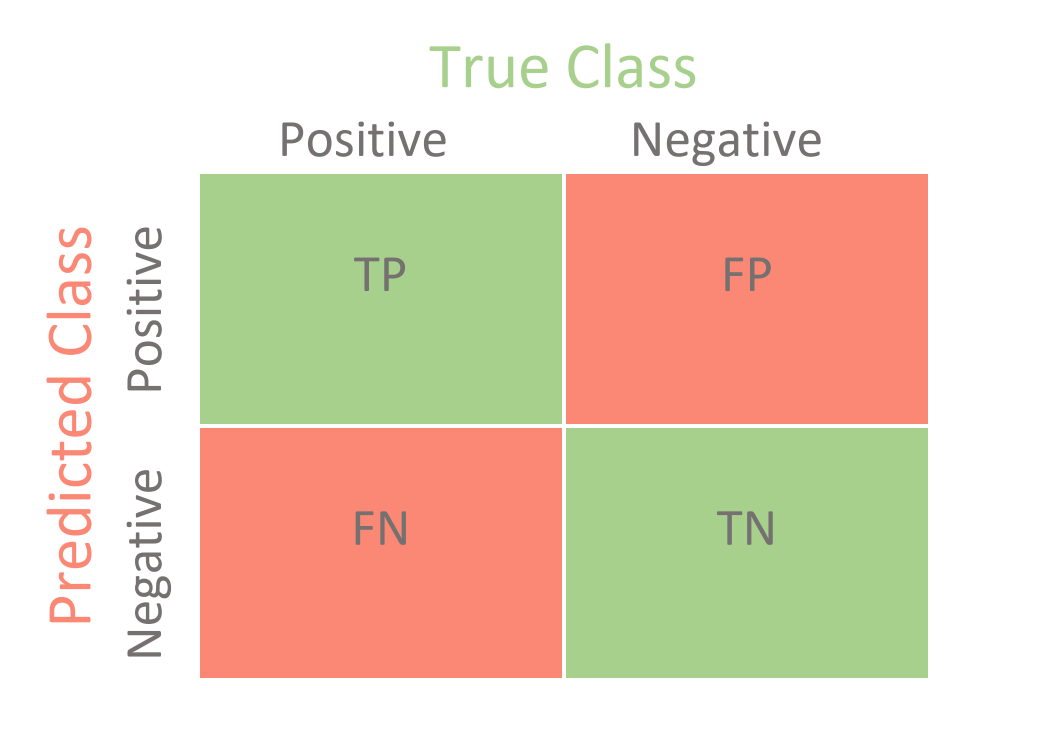
\includegraphics[width=0.7\columnwidth]{confusion_matrix.png} 
\end{center}

The project's confusion matrix:

\begin{tabularx}{0.8\textwidth} { 
  | >{\centering\arraybackslash}X 
  | >{\centering\arraybackslash}X 
  | >{\centering\arraybackslash}X | }
 \hline
 1018 & 4 \\
 \hline
 3 & 975  \\
\hline
\end{tabularx}

-
\newline
Interesting outcomes:
\newline
Precision: 0.9961
\newline
False Positive Rate: 0.0041
\newline
False Negative Rate: 0.0029
\newline
Recall: 0.9970

Loss visualization graph:

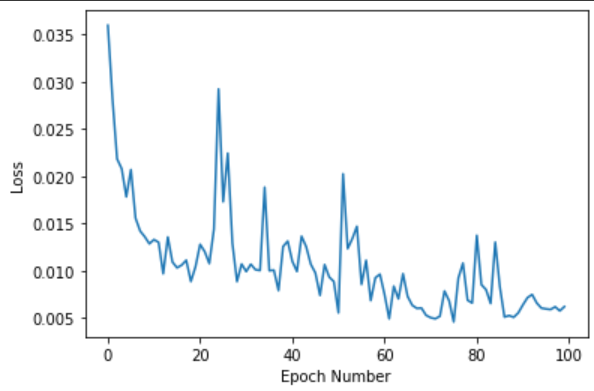
\includegraphics{Loss Visualization.png}
as we can see there were small spikes in the loss function's value during the learning process.
\newline
one can infer by looking at the graph that a smaller learning rate could have been better. For the sake of learning, I placed this graph here, despite the fact that a simple parameter change could make the graph slightly prettier.

\section{Discussion}
It seems that this exercise has deemed neural networks full of potential, for even an incredibly simple network was able to achieve amazing results (as one can see in the third section).
\newline
In the exercise we experimented with forward and back propagation, rather than just understanding the theory behind, as they were our methods to better train our model.
\newline
We have examined how a neural network is set up and used a simple neural network to derive the values at each node during the forward pass.

The Gradient descent which is a well known and commonly used to train machine learning models, was used as well.
\newline
As a final note, I would like to point out that a non-fixed learning rate could have both saved processing power and help us reach better results.

The former would have been achieved by using a rather large learning rate in the beginning, while the latter could have taken effect by lowering the learning rate as we get closer to the final result (we can see that the loss function in the last epochs increases and decreases repeatedly).

\section{Code}

link to our google colab notebook: 

\url{https://colab.research.google.com/drive/1fVHjdTyuftUrxYa2Jz6M9LMbX3SMCXff?usp=share_link}

\bibliographystyle{plain}
\bibliography{references}
\end{document}